
\section{Análisis de convergencia}

Es necesario comprobar el correcto funcionamiento del algoritmo de resolución del problema de Línea Sustentadora. Para ello se lleva a cabo un análisis de convergencia de varios coeficientes en función del número de paneles de discretización $\left( n \right)$. 

Las variables de estudio son el coeficiente de sustentación y el coeficiente de momento respecto del LE a ángulos de ataque de $0 \degrees$ y $5 \degrees$. Estos coeficientes se calculan para discretizaciones con $N$ en el rango $1$--$200$. Las propiedades geométricas y aerodinámicas del ala volante son las presentadas hasta el momento. En la figura \ref{fig:convergence_analysis} se muestran los resultados obtenidos. No es posible calcular el error relativo en las variables de estudio, pues no se conoce su valor real.

\begin{figure}[ht]
    \centering
    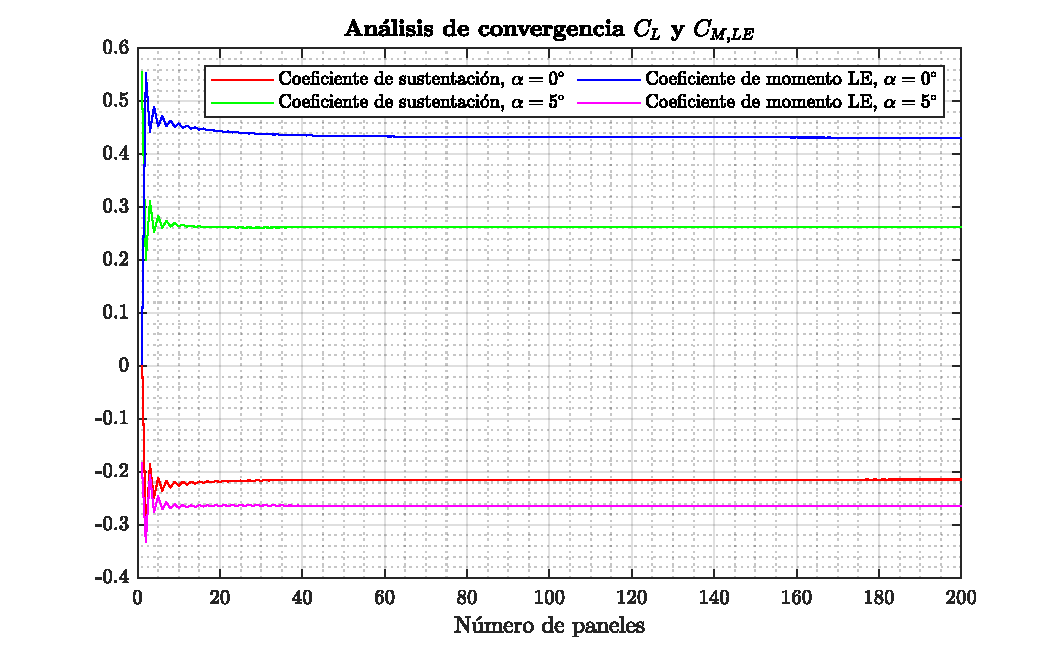
\includegraphics[width=\linewidth]{imagenes/analisis_convergencia/convergence_analysis.pdf}
    \caption{Coeficiente de sustentación $\left( C_L \right)$ y coeficiente de momentos respecto de LE $\left( C_{M,LE} \right)$ a $\alpha = 0 \degrees$ y $5\degrees$, en función del número de paneles $\left( N \right)$.}
    \label{fig:convergence_analysis}
    \vspace{-4mm}
\end{figure}

Para $N < 40$ se aprecian oscilaciones importantes en los coeficientes estudiados. Para $N > 80$ las cuatro variables de estudio alcanzan a su valor final. Para $80 < N \leq 200$ no se observan cambios en sus valores, estabilizándose por completo. 

Puede concluirse que las variables de estudio convergen para una discretización con $N \approx 100$. Dada la linealidad del problema, el $C_L$, $C_{M,LE}$ y otras variables derivadas, \eg, el centro de presiones $\left( x_{cp} \right)$ convergen también para otros ángulos de ataque. 